% Cluster D: the repaired slit lemma and the exact free-component criterion
% Body-only LaTeX; uses only preamble macros and fixed cross-cluster labels.

\section{The exact free-component criterion}\label{sec:criterion}

Theorem~\ref{thm:realization} converts a protected ribbon-routing certificate into an
actual carrier, but it leaves open the question of when such a certificate exists: the
embedded finite tree of Definition~\ref{def:certificate} looks like an arbitrary choice,
and one might fear that its existence depends on delicate features of the atoms or of the
forbidden data. The present section removes the arbitrary tree choice. We prove that the
existence of a protected ribbon-routing certificate is governed by a single, exact,
purely planar condition: one component of a frozen free domain must reach every required
atom by a singleton port. The section carries the one intentional mathematical divergence
of this paper from the source manuscript \cite{MWman}: the slit lemma below is stated and
proved in a repaired form, and the proof of the criterion is rewritten to match. The
divergence is recorded precisely in Remark~\ref{rem:repair}.

\subsection{The frozen free domain}\label{subsec:D-frozen}

Freeze the complete finite future inventory before choosing a connector. Concretely, let
$U$ be the Jordan localization and let $Q\subset U$ be the union of
all root-shadow atoms $A_1,\dots,A_s$, the closed terminal protected collars of every
protected prime-end chain in the inventory, the separated obstacles, the critical-value
exclusion, and the localization-forbidden set. As a standing convention, following the
compact-containment hypotheses of the certificate setup, we assume each constituent of
$Q$ is closed in $U$ and that the atoms, collars, and obstacles are compactly contained
in $U$; this guarantees that the free domain defined next is open. Put
\begin{equation}\label{eq:D-free-domain}
\Omfree \;=\; U\setminus Q
\end{equation}
(equation~(9.4) of the manuscript \cite{MWman}). The set $\Omfree$ is open, and its
connected components are plane domains, the \emph{free components} of the frozen data.

A component $\Omega_0$ of $\Omfree$ \emph{has simultaneous singleton ports} to the
required atoms if there are pairwise disjoint Jordan arcs
$\alpha_1,\dots,\alpha_s\colon[0,1]\to U$ such that, for every $i$, the arc $\alpha_i$
meets $A_i$ exactly in the single point $x_i=\alpha_i(0)$ and satisfies
$\alpha_i\bigl((0,1]\bigr)\subset\Omega_0$. The landing point $x_i$ is called a
\emph{free point} of $A_i$ because it is reached from the free domain; no further
property of $x_i$ is assumed at this stage. (Compare the unprotected exposure loci of
Lemma~\ref{lem:port-localization}, where an additional protected-impression exclusion is
imposed; the interaction between the two notions is illustrated in
Example~\ref{ex:no-common-component} below.)

The adjective \emph{frozen} is load-bearing, and we emphasize it once. The set $Q$ lists
the complete finite future inventory: every atom that will ever have to be joined, the
closed terminal collar of every protected chain that any future step of a proof will
read, every obstacle that must remain separated, the full critical-value exclusion, and
the localization-forbidden set. This list is fixed \emph{before} any connector is chosen.
Nothing may be added to $Q$ afterwards, and nothing may be removed from it; all later
monotone operations act on proposed connectors, never on the inventory. This discipline
is exactly what gives the criterion of Theorem~\ref{thm:free-component} its
if-and-only-if form, and what makes its failure clause persistent: a separation already
visible in the frozen data can never be talked away by enlarging a connector. The
horizon-first closure results of the manuscript \cite{MWman} address how such an
inventory stabilizes; here the inventory is simply given, finite, and immutable.

\subsection{The repaired slit lemma}\label{subsec:D-slits}

The sufficiency direction of the criterion rests on the fact that finitely many pairwise
disjoint one-ended slits do not disconnect a plane domain. This is Lemma~10.7 of the
manuscript. Its printed statement contains a formal inconsistency (a map into an open
domain cannot take a boundary value) together with an endpoint mismatch with its
intended application; both defects are repaired in the statement below, and
Remark~\ref{rem:repair} records the divergence. The mathematical core of the
manuscript's argument --- the transverse-rectangle detour around the free endpoint ---
is retained in full.

\begin{lemma}[One-ended slits do not disconnect a plane domain; manuscript Lemma 10.7,
repaired]\label{lem:slits}
Let $\Omega\subset\C$ be a domain and let
$\delta_1,\dots,\delta_s\colon[0,1]\to\overline{\Omega}$ be Jordan arcs with pairwise
disjoint images such that $\delta_i(0)\in\partial\Omega$ and
$\delta_i\bigl((0,1]\bigr)\subset\Omega$ for every $i$. Then
\[
\Omega\setminus\bigcup_{i=1}^{s}\delta_i\bigl((0,1)\bigr)
\]
is path connected; in particular every free endpoint $\delta_i(1)$ lies in this set and
can be joined inside it to every other point of it.
\end{lemma}

\begin{proof}
Call $\delta_i$ the \emph{$i$-th slit}, write
$\sigma_i:=\delta_i\bigl((0,1]\bigr)$ for its \emph{half-open} part and
$\sigma_i^{\circ}:=\delta_i\bigl((0,1)\bigr)$ for its \emph{open} part, and call
$\delta_i(1)$ its \emph{tip}. The set to be proved path connected is
$\Omega\setminus\bigcup_i\sigma_i^{\circ}$, which contains all $s$ tips. If $s=0$ there
is nothing to prove, so assume $s\ge1$; then $\partial\Omega\neq\varnothing$.

\emph{Step 0: two preliminary observations.}
First, each half-open part $\sigma_i$ is relatively closed in $\Omega$. Indeed, the
closure of $\sigma_i$ in $\C$ is the compact arc $\delta_i([0,1])$, so the only point of
$\overline{\sigma_i}\setminus\sigma_i$ is $\delta_i(0)\in\partial\Omega$, which does not
lie in $\Omega$. Consequently $\Omega\setminus\sigma_i$ is open. By contrast, the open
part $\sigma_i^{\circ}$ is \emph{not} relatively closed in $\Omega$: its closure inside
$\Omega$ also contains the tip $\delta_i(1)\in\Omega$. This distinction is precisely the
point at which the manuscript's induction required repair; the proof below removes the
half-open parts first and reattaches the tips afterwards.

Second, every Jordan arc in the plane is tame: it can be extended to a Jordan curve,
and the Schoenflies theorem then supplies a homeomorphism of $\C$ carrying the curve to
a round circle and the arc to a circular subarc, hence, after one more homeomorphism,
onto the straight segment $[0,1]\times\{0\}$; see, e.g.,
\cite{New51,Why42}. Since path connectivity is a topological invariant and a
homeomorphism of $\C$ carries domains to domains and boundaries to boundaries, we may
straighten any \emph{single} slit whenever convenient. (Straightening one slit will in
general bend the others; each step below straightens only the slit it is processing.)

\emph{Step 1: removing a single half-open slit leaves a domain.}
Let $\Omega$ be a domain and let $\delta$ be a single arc as in the statement, with
half-open part $\sigma=\delta\bigl((0,1]\bigr)$. We claim that
$\Omega':=\Omega\setminus\sigma$ is again a domain. Openness was proved in Step~0, so
only path connectivity is at issue. By tameness we may assume, after a homeomorphism of
$\C$, that
\[
\delta(t)=(t,0)\quad(0\le t\le1),
\]
so that $\Omega$ is a domain containing $S:=(0,1]\times\{0\}$, with
$(0,0)\in\partial\Omega$, and we must join two arbitrary points
$x,y\in\Omega\setminus S$ by a path in $\Omega\setminus S$.

\emph{(a) A polygonal start missing an initial tail.}
Since a plane domain is polygonally connected \cite{New51}, choose a polygonal path
$P\subset\Omega$ from $x$ to $y$. The path $P$ is compact and does not contain the
boundary point $(0,0)$, so
\[
r:=\dist\bigl((0,0),P\bigr)>0 .
\]
Fix $\varepsilon:=\tfrac12\min(r,1)$. Every point of the initial tail
$[0,\varepsilon]\times\{0\}$ lies within distance $\varepsilon<r$ of the origin, so $P$
misses $[0,\varepsilon]\times\{0\}$. This is the only part of the closed slit that a
compact subset of $\Omega$ cannot in general avoid by compactness alone: the closed slit
image leaves every compact subset of $\Omega$ only along points accumulating at
$\delta(0)=(0,0)\in\partial\Omega$, and near that end the continuity of $\delta$ at $0$
confines the slit to a small disk around the origin. The remaining part
$\delta([\varepsilon,1])=[\varepsilon,1]\times\{0\}$ is a compact subset of $\Omega$ and
will be handled by explicit detours.

\emph{(b) A thin rectangle around the compact subarc.}
The segment $[\varepsilon,1]\times\{0\}$ lies in $\Omega$, and $(1,0)\in\Omega$ is an
interior point of $\Omega$; hence there is $\eta\in(0,\tfrac12)$ with
$[1,1+\eta]\times\{0\}\subset\Omega$. The segment
$L:=[\varepsilon/2,\,1+\eta]\times\{0\}$ is then a compact subset of $\Omega$, so
$\dist(L,\C\setminus\Omega)>0$, and we may choose
$h\in\bigl(0,\min(\varepsilon/2,\dist(L,\C\setminus\Omega)/2)\bigr)$ and set
\[
R:=[\varepsilon/2,\,1+\eta]\times[-h,h]\subset\Omega .
\]
The rectangle $R$ meets the closed slit $[0,1]\times\{0\}$ exactly in the core
$c:=[\varepsilon/2,\,1]\times\{0\}$: the slit enters $R$ through the midpoint of its
left short side and terminates at the tip $(1,0)$, an interior point of $R$. In
particular $R\cap S=[\varepsilon/2,1]\times\{0\}=c$.

We record the key connectivity property of the slit rectangle: \emph{$R\setminus c$ is
path connected.} Indeed, let $V:=\{1+\eta/2\}\times[-h,h]$, a vertical segment in $R$
missing $c$. A point of $R\setminus c$ with ordinate $y\neq0$ travels horizontally to
the point of $V$ with the same ordinate; the horizontal path misses the axis
$\mathbb{R}\times\{0\}$ entirely, hence misses $c$. A point of $R\setminus c$ with
ordinate $0$ has abscissa in $(1,1+\eta]$ and travels along the axis to $(1+\eta/2,0)$;
this path keeps abscissa $>1$, hence misses $c$. Since $V$ is connected, the claim
follows. Geometrically: the two long sides of $R$ are joined to each other inside
$R\setminus c$ \emph{around the tip}, by crossing the axis at abscissae beyond $1$.

\emph{(c) Transverse perturbation and detour repair.}
Perturb the interior vertices of $P$, keeping the endpoints $x,y$ fixed, so that no
interior vertex lies on the axis $\mathbb{R}\times\{0\}$ and no edge of $P$ is collinear
with the axis; if an endpoint happens to lie on the axis (necessarily off $S$), perturb
its adjacent vertex so that the incident edge is not horizontal. Since $P$ is compact
with $\dist(P,\C\setminus\Omega)>0$ and $\dist\bigl(P,[0,\varepsilon]\times\{0\}\bigr)
\ge r-\varepsilon>0$, a sufficiently small such perturbation keeps $P$ inside $\Omega$
and away from the initial tail. After the perturbation, every edge of $P$ meets the axis
in at most one point, and every meeting point interior to an edge is a transverse
crossing. Hence $P$ meets $S$ in finitely many points, all of the form $P(t_j)$ with
parameters $0<t_1<\dots<t_m<1$ interior to edges, and all lying in
$( \varepsilon,1]\times\{0\}\subset\Int R$. (If $m=0$, the path $P$ already joins $x$ to
$y$ in $\Omega\setminus S$ and Step~1 is complete.)

By transversality, for each $j$ there is $\rho_j>0$ such that the parameter interval
$[t_j-\rho_j,\,t_j+\rho_j]$ has image in $\Int R$, meets the axis only at $t_j$, and the
two punctured halves of the image lie strictly on opposite sides of the axis; shrink the
$\rho_j$ so that these intervals are pairwise disjoint and avoid $0$ and $1$. Put
$p_j^{-}:=P(t_j-\rho_j)$ and $p_j^{+}:=P(t_j+\rho_j)$; both lie in $R\setminus c$.
Now modify $P$ as follows: on each interval $[t_j-\rho_j,\,t_j+\rho_j]$, replace the
sub-path of $P$ by a path from $p_j^{-}$ to $p_j^{+}$ inside $R\setminus c$, which
exists by (b); keep $P$ unchanged elsewhere. Each detour lies in $R\subset\Omega$ and
misses $S$, because $S\cap R=c$ and the detour misses $c$, while $S\setminus R$ is
disjoint from $R$. The unchanged pieces of $P$ carry parameters outside the intervals
$(t_j-\rho_j,\,t_j+\rho_j)$ and therefore avoid $S$, since the crossings $t_j$ were the
only parameters at which $P$ met $S$. The concatenation is a path from $x$ to $y$ in
$\Omega\setminus S$.

Observe that each detour crosses the axis only at abscissae strictly beyond $1$: it
travels \emph{around} the tip, through points arbitrarily close to $\delta(1)$ but never
through any point of the closed slit; the tip itself, which here has been removed
together with the rest of $\sigma$, is not needed as a way-station. This completes
Step~1: $\Omega'=\Omega\setminus\sigma$ is a domain.

\emph{Step 2: removing all half-open slits leaves a domain.}
Set $\Omega_{(0)}:=\Omega$ and, inductively,
$\Omega_{(j)}:=\Omega_{(j-1)}\setminus\sigma_j$ for $1\le j\le s$. We claim that each
$\Omega_{(j)}$ is a domain and that $\delta_j$ is a one-ended slit of $\Omega_{(j-1)}$
in the sense of the statement. Indeed, suppose $\Omega_{(j-1)}$ is a domain. Because the
slit images are pairwise disjoint, $\sigma_j$ is disjoint from
$\sigma_1,\dots,\sigma_{j-1}$, so $\sigma_j\subset\Omega_{(j-1)}$. The point
$\delta_j(0)$ lies outside $\Omega\supset\Omega_{(j-1)}$, and it is the limit of the
points $\delta_j(t)\in\Omega_{(j-1)}$ as $t\downarrow0$; hence
$\delta_j(0)\in\partial\Omega_{(j-1)}$ and
$\delta_j\colon[0,1]\to\overline{\Omega_{(j-1)}}$. Step~1, applied to the domain
$\Omega_{(j-1)}$ and the single slit $\delta_j$, now shows that $\Omega_{(j)}$ is a
domain. After $s$ steps we conclude: the set
\[
\Omega_{(s)}\;=\;\Omega\setminus\bigcup_{i=1}^{s}\sigma_i
\;=\;\Omega\setminus\bigcup_{i=1}^{s}\delta_i\bigl((0,1]\bigr)
\]
is open and path connected.

\emph{Step 3: reattaching the tips.}
The set whose path connectivity is asserted differs from $\Omega_{(s)}$ exactly by the
$s$ tips:
\[
\Omega\setminus\bigcup_{i=1}^{s}\sigma_i^{\circ}
\;=\;\Omega_{(s)}\,\cup\,\{\delta_1(1),\dots,\delta_s(1)\},
\]
and the tips are pairwise distinct points not in $\Omega_{(s)}$. Since $\Omega_{(s)}$ is
path connected, it suffices to join each tip to some point of $\Omega_{(s)}$ by a path
which, apart from the tip itself, lies in $\Omega_{(s)}$.

Fix $i$ and straighten the $i$-th slit: let $\Phi$ be a homeomorphism of $\C$ with
$\Phi\bigl(\delta_i([0,1])\bigr)=[0,1]\times\{0\}$ and $\Phi(\delta_i(t))=(t,0)$. The
union $K:=\bigcup_{k\neq i}\delta_k([0,1])$ of the other closed slit images is compact
and disjoint from $\delta_i([0,1])$, so $\Phi(K)$ is compact and disjoint from
$[0,1]\times\{0\}$. The model tip $(1,0)$ lies in the open set $\Phi(\Omega)$ and
outside the closed set $\Phi(K)$, so
\[
\mu:=\dist\Bigl((1,0),\,\Phi(K)\cup\bigl(\C\setminus\Phi(\Omega)\bigr)\Bigr)>0 .
\]
Choose $a\in\bigl(0,\min(\mu/2,\tfrac12)\bigr)$ and consider the square
$R_i:=[1-a,\,1+a]\times[-a,a]$. Every point of $R_i$ lies within distance $a\sqrt2<\mu$
of the model tip, so $R_i\subset\Phi(\Omega)$ and $R_i\cap\Phi(K)=\varnothing$; moreover
$R_i$ meets the model slit $[0,1]\times\{0\}$ exactly in $[1-a,1]\times\{0\}$. The
\emph{escape segment}
\[
E_i:=[1,\,1+a/2]\times\{0\}
\]
runs from the model tip into $R_i$; every point of $E_i$ other than the tip has abscissa
$>1$, hence lies on none of the straightened slits, and lies in $R_i$, hence off
$\Phi(K)$. Pulling back, $\beta_i:=\Phi^{-1}(E_i)$ is a Jordan arc from $\delta_i(1)$ to
a point $z_i\in\Omega_{(s)}$ with $\beta_i\setminus\{\delta_i(1)\}\subset\Omega_{(s)}$.
Thus the tip $\delta_i(1)$ lies in the same path component as $z_i$, hence in the path
component of $\Omega_{(s)}$.

The same square makes the two-sided accessibility of the tip transparent: inside
$R_i\setminus\bigl([1-a,1]\times\{0\}\bigr)$ the two long sides of $R_i$ are joined
around the tip by the vertical segment at abscissa $1+a/2$, so the tip is accessible
from either side of the slit, and both accesses land in one and the same path component
of the complement. Finally, note that the escape arc $\beta_i$ can be made arbitrarily
small: shrinking $a$ shrinks $E_i$ to the model tip, and continuity of $\Phi^{-1}$ then
confines $\beta_i$ to any prescribed neighborhood of $\delta_i(1)$.

\emph{Step 4: conclusion.}
By Steps 2 and 3 the set
$\Omega\setminus\bigcup_i\sigma_i^{\circ}=\Omega_{(s)}\cup\{\delta_1(1),\dots,
\delta_s(1)\}$ is path connected, and it contains every free endpoint $\delta_i(1)$;
each of these can therefore be joined inside it to every other point of it.
\end{proof}

Two by-products of the proof will be used in the proof of
Theorem~\ref{thm:free-component} and are worth recording explicitly. First, by Step~2,
removing the \emph{half-open} slits $\delta_i((0,1])$ leaves an open, path connected
set --- indeed a plane domain, hence a polygonally connected one. Second, by Step~3,
every tip $\delta_i(1)$ admits arbitrarily small escape arcs: for every neighborhood $N$
of $\delta_i(1)$ there is a Jordan arc $\beta\subset N$ from $\delta_i(1)$ into the slit
complement with $\beta\setminus\{\delta_i(1)\}\subset
\Omega\setminus\bigcup_k\delta_k\bigl((0,1]\bigr)$.

\begin{remark}[The repair]\label{rem:repair}
We record the divergence from the printed manuscript statement \cite{MWman}. Manuscript
Lemma~10.7 states the hypothesis in the form
$\delta_i\colon[0,1]\to\Omega$ with $\delta_i(0)\in\partial\Omega$, which is formally
inconsistent: a map into the open domain $\Omega$ cannot take a boundary value. It then
removes the half-open slits $\delta_i\bigl((0,1]\bigr)$, \emph{including} the free
endpoints $\delta_i(1)$, while the manuscript's proof of Theorem~10.8 (reproduced as
Theorem~\ref{thm:free-component} below) joins precisely those outer endpoints by paths
inside the complement --- an endpoint mismatch: the points to be joined have just been
deleted. The statement of Lemma~\ref{lem:slits} repairs both defects at once: the
codomain is $\overline{\Omega}$, so the initial boundary value is legitimate, and only
the open arcs $\delta_i\bigl((0,1)\bigr)$ are removed, so the free endpoints remain
available for routing.

A third, smaller point is repaired inside the proof. The manuscript's induction asserts
that the removed slit is relatively closed in $\Omega$, so that the complement is again
a domain and the one-slit argument iterates. For the half-open slit
$\delta_i\bigl((0,1]\bigr)$ this is true (Step~0), but for the open slit
$\delta_i\bigl((0,1)\bigr)$ it is false: the closure inside $\Omega$ adds the tip, so
the complement of the open slit is not open at the tip and the inductive step cannot be
applied verbatim to the repaired statement. The proof above therefore removes the
half-open slits one at a time (Steps~1 and~2), where relative closedness does hold, and
reattaches the $s$ retained tips afterwards by the tip-accessibility argument (Step~3).

The repair changes no application. Every invocation of the lemma in the source
manuscript --- and every invocation in this paper --- uses exactly the repaired form:
the slits to be removed are open port interiors, and the retained outer endpoints are
then joined inside the complement. The transverse-rectangle detour, which is the
mathematical core of the manuscript's one-slit argument, is unchanged.
\end{remark}

\subsection{The criterion}\label{subsec:D-criterion}

\begin{theorem}[Protected Free-Component Criterion; manuscript Theorem 10.8]
\label{thm:free-component}
A protected ribbon-routing certificate exists if and only if one component of $\Omfree$
has simultaneous singleton ports to every required atom. If a first protected collar or
obstacle separates two required port classes, no further monotone connector enlargement
inside the current localization can repair the failure.
\end{theorem}

\begin{proof}
\emph{Necessity.}
Let a protected ribbon-routing certificate be given, with free-port arcs
$\alpha_1,\dots,\alpha_s$, landing points $x_i=\alpha_i(0)\in A_i$, and embedded finite
tree $G$ joining the outer port endpoints (Definition~\ref{def:certificate}). Delete the
atoms from the connector and consider
\[
X\;:=\;G\,\cup\,\bigcup_{i=1}^{s}\alpha_i\bigl((0,1]\bigr).
\]
The tree $G$ is connected, and each half-open port arc $\alpha_i\bigl((0,1]\bigr)$ is a
connected set containing the outer endpoint $\alpha_i(1)\in G$; hence $X$ is connected.
Moreover $X\subset\Omfree$: by Definition~\ref{def:certificate}, the sets
$\alpha_i\bigl((0,1]\bigr)$ and $G$ lie in $U$ and avoid every atom, the obstacle and
critical-value set, and every closed terminal protected collar.  The
localization-forbidden data are avoided by the frozen-inventory discipline: the
manuscript treats them as part of the forbidden set that certificate data must miss, and
we adopt the same reading here.  The avoided sets are exactly the constituents of $Q$. A
connected subset of the open set $\Omfree$ lies in a single component $\Omega_0$. The
certificate's own port arcs are then simultaneous singleton ports of $\Omega_0$: they
are pairwise disjoint Jordan arcs, $\alpha_i$ meets $A_i$ exactly in $\{x_i\}$, and
$\alpha_i\bigl((0,1]\bigr)\subset X\subset\Omega_0$.

\emph{Sufficiency.}
Conversely, let $\Omega_0$ be a component of $\Omfree$ with simultaneous singleton ports
$\alpha_1,\dots,\alpha_s$. Fix $\tau\in(0,1]$ and shorten each port away from the atoms,
replacing $\alpha_i$ by its initial subarc $\alpha_i|_{[0,\tau]}$, reparametrized over
$[0,1]$ and still denoted $\alpha_i$; the shortened arcs remain pairwise disjoint
simultaneous singleton ports, and the shortening emphasizes that only the germ of each
port at its atom matters. Write $y_i:=\alpha_i(1)$ for the retained outer endpoints.

The shortened ports are one-ended slits of the domain $\Omega_0$ in the sense of
Lemma~\ref{lem:slits}. Indeed, their images are pairwise disjoint; the interiors satisfy
$\alpha_i\bigl((0,1]\bigr)\subset\Omega_0$; and the landing point
$x_i=\alpha_i(0)$ lies in $A_i\subset Q$, hence outside $\Omega_0$, while being the
limit of the points $\alpha_i(t)\in\Omega_0$, so that $x_i\in\partial\Omega_0$ and
$\alpha_i\colon[0,1]\to\overline{\Omega_0}$. The retained port interiors are therefore
finitely many pairwise disjoint one-ended slits of $\Omega_0$, and
Lemma~\ref{lem:slits} applies to remove their \emph{open} parts: the set
\[
W\;:=\;\Omega_0\setminus\bigcup_{i=1}^{s}\alpha_i\bigl((0,1)\bigr)
\]
is path connected, and it contains the outer endpoints $y_1,\dots,y_s$ --- which is
exactly what the repaired statement guarantees.

We now upgrade the joining paths supplied by path connectivity of $W$ to an embedded
polygonal tree, using the two by-products recorded after the proof of
Lemma~\ref{lem:slits}. First, by Step~2 of that proof,
\[
\Omega'\;:=\;\Omega_0\setminus\bigcup_{i=1}^{s}\alpha_i\bigl((0,1]\bigr)
\]
is a plane domain. Second, by Step~3, each tip $y_i$ admits arbitrarily small escape
arcs into $\Omega'$. If $s=1$, the single shortened port together with the degenerate
one-vertex tree $\{z_1\}$, obtained from any escape arc, is already a certificate, so
assume $s\ge2$. Let $\rho:=\tfrac13\min_{i\neq j}|y_i-y_j|>0$, and choose for each
$i$ an escape arc $\beta_i\subset B(y_i,\rho)$ with $\beta_i(0)=y_i$ and
$\beta_i\bigl((0,1]\bigr)\subset\Omega'$; the balls $B(y_i,\rho)$ are pairwise
disjoint, so the arcs $\beta_i$ are pairwise disjoint. Put $z_i:=\beta_i(1)\in\Omega'$.

Since the domain $\Omega'$ is polygonally connected, choose polygonal paths
$P_2,\dots,P_s\subset\Omega'$ joining $z_1$ to $z_2,\dots,z_s$. Perturb them, keeping
their endpoints fixed, into general position inside $\Omega'$: after an arbitrarily
small perturbation, any two edges taken from distinct paths, or nonadjacent edges of one
path, meet in at most one point and transversely, and no vertex of one path lies on
another path except at shared endpoints. The union $\Gamma:=P_2\cup\dots\cup P_s$ is
then a connected finite plane graph in $\Omega'$ containing $z_1,\dots,z_s$: its
vertices are the path endpoints together with the finitely many transverse crossings, at
which we subdivide. Let $G_0\subset\Gamma$ be an inclusion-minimal connected subgraph
containing $\{z_1,\dots,z_s\}$. Then $G_0$ is a finite tree: were it to contain a
cycle, deleting one edge of the cycle would leave a connected subgraph still containing
every $z_i$, contradicting minimality. Being a subgraph of an embedded graph, $G_0$ is
embedded, and $G_0\subset\Omega'$.

The escape arcs may meet $G_0$ before their endpoints, so we trim them by a first-hit
argument. For each $i$ the set $\{t\in[0,1]:\beta_i(t)\in G_0\}$ is closed, and it is
nonempty because $\beta_i(1)=z_i\in G_0$; let $t_i^{*}$ be its minimum. Since
$\beta_i(0)=y_i\notin\Omega'\supset G_0$ we have $t_i^{*}>0$. Set
$\beta_i':=\beta_i|_{[0,t_i^{*}]}$ and $z_i':=\beta_i(t_i^{*})\in G_0$, so that
$\beta_i'\cap G_0=\{z_i'\}$.

Assemble the certificate. Define the rerouted port arcs
$\tilde\alpha_i:=\alpha_i*\beta_i'$ for $1\le i\le s$, the concatenation of $\alpha_i$
and $\beta_i'$, reparametrized over $[0,1]$. Each $\tilde\alpha_i$ is a Jordan arc: both
pieces are Jordan arcs meeting exactly at $y_i=\alpha_i(1)=\beta_i'(0)$, because
$\beta_i'\setminus\{y_i\}\subset\Omega'$ while the image
$\alpha_k([0,1])$ of every port lies in
$Q\cup\bigcup_j\alpha_j\bigl((0,1]\bigr)$, a set disjoint from $\Omega'$. The same
disjointness, together with the pairwise disjoint balls containing the $\beta_i$, shows
that $\tilde\alpha_1,\dots,\tilde\alpha_s$ are pairwise disjoint. Each $\tilde\alpha_i$
meets $A_i$ exactly in $\{x_i\}$, and its interior satisfies
$\tilde\alpha_i\bigl((0,1]\bigr)\subset\Omega_0\subset\Omfree$: it avoids every atom,
every closed terminal protected collar, the obstacle and critical-value set, and the
localization-forbidden set --- exactly the avoidance clauses that
Definition~\ref{def:certificate} imposes on free-port arcs. Next, subdivide $G_0$ so
that each $z_i'$ is a vertex, and call the resulting embedded finite tree $G$. Then
$G\subset\Omega'$ avoids the same forbidden sets, joins the outer port endpoints
$z_1',\dots,z_s'$, and meets each port arc $\tilde\alpha_i$ exactly in its outer
endpoint $z_i'$, by the first-hit property and $G\subset\Omega'$. Consequently
$G\cup\bigcup_i\tilde\alpha_i$ is again a finite tree: it is connected, and attaching
finitely many pairwise disjoint arcs to a tree, each along a single endpoint, adds one
vertex and one edge at a time and so preserves the tree characterization
$(\text{vertices})-(\text{edges})=1$ for connected finite graphs. The planar cyclic
order of half-edges at every vertex is the one induced by the embedding, and it is
retained as the certificate's ribbon datum. Finally, the protected prime-end crosscut
chains, with their pairwise disjoint closed terminal collars, belong to the frozen
inventory and are avoided as recorded above. All clauses of
Definition~\ref{def:certificate} are satisfied: the rerouted ports $\tilde\alpha_i$
together with the spanning tree $G$ constitute a protected ribbon-routing certificate.
Theorem~\ref{thm:realization} now realizes it by a compact connected full carrier with
singleton attachment traces, protected crosscut survival, and preserved cyclic order.

\emph{Persistence.}
For the final assertion, suppose that at some stage of the frozen inventory a first
protected collar or obstacle $C_0\subset Q$ separates two required port classes: after
the insertion of $C_0$, every component of $\Omfree$ admitting a singleton port to
$A_i$ is distinct from every component admitting a singleton port to $A_j$, for some
pair of required atoms $A_i,A_j$. Then no single component has simultaneous singleton
ports to both atoms, so by the criterion just proved no protected ribbon-routing
certificate exists. This failure is permanent under monotone connector enlargement
inside the current localization, for two cumulative reasons. First, enlargement acts on
proposed connectors, never on the inventory: $Q$ is frozen, so $\Omfree$ and its
partition into components are unchanged, and the necessity argument applies verbatim to
every enlarged connector --- its routing part is a connected set which, were the
certificate discipline respected, would lie in one component of $\Omfree$ while porting
to atoms in two different components; this is impossible, since a connected subset of
$U\setminus Q$ lies in a single component. Second, the only way for a connected set to
join the two components is to meet $Q$ across the separating part, and if that part is
protected or forbidden, the intersection itself violates the certificate: absorbing a
protected collar erases the protected access it certifies, and meeting an obstacle or
the critical-value exclusion is excluded outright. (Compare
Proposition~\ref{prop:access-collision} for an analytic incarnation of the first
mechanism.) Hence no further monotone connector enlargement inside the current
localization can repair the failure; the only conceivable cure --- deleting the
separator $C_0$ from the inventory --- is a revision of the frozen data, which the
formalism forbids.
\end{proof}

The construction is natural under univalent changes of the Jordan localization. An
orientation-preserving conformal homeomorphism of Jordan disks extends over the Jordan
boundaries, and it carries the frozen set $Q$, the free domain \eqref{eq:D-free-domain}
and its components, the port arcs, the escape arcs, and the spanning tree to their
transported counterparts; the transported data form a certificate for the transported
inventory, and the realized carriers correspond as in
Proposition~\ref{prop:naturality}. At the same time the criterion is qualitative: the
number of ports and of ribbon sides is not bounded uniformly, and no width, modulus, or
incidence estimate enters at any point. Nothing in this section constructs the frozen
inventory of a dynamical situation; the corresponding virtual free-component questions
are stated in the source manuscript only as open problems \cite{MWman}, and no part of
this paper bears on them.

\subsection{A separator between individually accessible atoms}\label{subsec:D-example}

The criterion of Theorem~\ref{thm:free-component} is strictly stronger than every
atom-by-atom access condition. The following example, promised in the introduction,
exhibits two atoms each of which passes every individual-access audit, while no common
free component exists; it is the minimal model of the failure mode that the persistence
clause certifies. See Figure~\ref{fig:separation}.

\begin{example}[Individual accesses without a common free component]
\label{ex:no-common-component}
Let $U:=\{z\in\C:|z|<2\}$ and take the two atoms
\[
A_1:=\bigl[-\tfrac14,\tfrac14\bigr],
\qquad
A_2:=\bigl[\tfrac54,\tfrac74\bigr],
\]
closed segments of the real axis, each a full continuum compactly contained in $U$.
Freeze exactly one further inventory item, the round circle
\[
C:=\{z:|z|=1\},
\]
recorded as a separated obstacle; all that matters below is that $C\subset Q$, so any
recording of $C$ in the frozen inventory would do. There
are no critical values and no further forbidden data, so the frozen set is
$Q=A_1\cup A_2\cup C$ and
\[
\Omfree=U\setminus(A_1\cup A_2\cup C).
\]

\emph{The free domain has exactly two components, one per atom.} Write
\[
\Omega_{\mathrm{in}}:=\{|z|<1\}\setminus A_1,
\qquad
\Omega_{\mathrm{ann}}:=\{1<|z|<2\}\setminus A_2,
\]
so that $\Omfree=\Omega_{\mathrm{in}}\sqcup\Omega_{\mathrm{ann}}$, a disjoint union of
open sets separated by the circle $C$. Each is connected, by an explicit radial--angular
path argument. In $\Omega_{\mathrm{in}}$, every point can be joined to the circle
$\{|z|=\tfrac12\}$, which misses $A_1$: a point with $\arg z\notin\{0,\pi\}$ travels
radially to modulus $\tfrac12$, and the radial path keeps its argument, hence stays off
the real axis and misses the real segment $A_1$; a real point of
$\Omega_{\mathrm{in}}$ has modulus in $(\tfrac14,1)$ and travels radially to modulus
$\tfrac12$ through real points of modulus $>\tfrac14$, which also miss $A_1$. In
$\Omega_{\mathrm{ann}}$, every point can be joined to the circle $\{|z|=\tfrac98\}$,
which misses $A_2$: a point with $\arg z\neq0$ travels radially inward keeping its
argument; a positive real point of $\Omega_{\mathrm{ann}}$ has modulus in
$(1,\tfrac54)\cup(\tfrac74,2)$, and in the first case it travels radially inward to
modulus $\tfrac98$ through positive real points of modulus $<\tfrac54$, while in the
second case it first travels along its own circle $\{|z|=\mathrm{const}\}$ (which
misses $A_2$, as $\tfrac74<|z|<2$) to argument $\pi$ and then proceeds radially inward
as before. Both sets are
therefore domains, and they are exactly the two components of $\Omfree$.

\emph{Every individual-access audit passes.} Exhibit the singleton ports
\[
\alpha_1(t):=\tfrac14+\tfrac t2,
\qquad
\alpha_2(t):=\tfrac74+\tfrac t8
\qquad(0\le t\le1):
\]
the arc $\alpha_1$ runs from $x_1=\tfrac14\in A_1$ to $\tfrac34$ and meets $A_1$ only at
$x_1$, with $\alpha_1\bigl((0,1]\bigr)=(\tfrac14,\tfrac34]\subset\Omega_{\mathrm{in}}$;
the arc $\alpha_2$ runs from $x_2=\tfrac74\in A_2$ to $\tfrac{15}8$ and meets $A_2$ only
at $x_2$, with
$\alpha_2\bigl((0,1]\bigr)=(\tfrac74,\tfrac{15}8]\subset\Omega_{\mathrm{ann}}$. Thus
each atom has a singleton port into \emph{its own} free component. In the language of
the port audit, with empty protected marking and with the atoms as their own completed
packets, both unprotected exposure loci are nonempty, so the hypotheses of
Lemma~\ref{lem:port-localization} hold and its conclusion is correct: the two arcs can
be (and are) chosen pairwise disjoint with interiors in the common complement of the
packets. Atom by atom, nothing is wrong.

\emph{No common free component exists.} Every port of $A_1$ runs in
$\Omega_{\mathrm{in}}$: if $\alpha$ is an arc with
$\alpha\cap A_1=\{\alpha(0)\}$ and $\alpha((0,1])$ contained in one component of
$\Omfree$, then $\alpha(t)\to\alpha(0)\in A_1\subset\{|z|\le\tfrac14\}$ forces
$|\alpha(t)|<1$ for small $t$, so the component is $\Omega_{\mathrm{in}}$. Likewise
every port of $A_2$ runs in $\Omega_{\mathrm{ann}}$, since points of $\Omfree$ near
$A_2$ have modulus in $(1,2)$. As $\Omega_{\mathrm{in}}\neq\Omega_{\mathrm{ann}}$, no
component of $\Omfree$ has simultaneous singleton ports to both atoms, and
Theorem~\ref{thm:free-component} yields: \emph{no protected ribbon-routing certificate
exists} for this frozen inventory. By the persistence clause, the failure is permanent:
the separator $C$ is the first (indeed the only) separating insertion, the two required
port classes are $\{\Omega_{\mathrm{in}}\}$ and $\{\Omega_{\mathrm{ann}}\}$, and no
monotone connector enlargement inside $U$ can repair the separation. The only cure
would be to delete $C$ from the frozen inventory --- a revision of the frozen data,
which the formalism forbids.
\end{example}

The example separates two layers of the theory cleanly. The hypotheses of
Lemma~\ref{lem:port-localization} --- individual exposure of every atom --- are
statements about each atom in isolation, and they hold here; the criterion of
Theorem~\ref{thm:free-component} is a statement about one common component, and it
fails. This is also precisely why Definition~\ref{def:packet} demands that the
completed packets be pairwise disjoint \emph{and cover $Q$}: the separator $C$ must be
assigned to some packet, and every typed assignment then exhibits a persistent defect
of the audit of Theorem~\ref{thm:audit}. Assigning $C$ to a separated-obstacle packet
gives $\Fill(C)=\{|z|\le1\}\supset A_1$, a packet merger with the completed packet of
$A_1$. Assigning $C$ to the atom seed of $A_2$ (necessarily together with a connecting
arc, to keep the seed connected) again puts the closed unit disk, hence $A_1$, inside
the completed packet of $A_2$: the same merger. Assigning $C$ to the atom seed of $A_1$
produces a completed packet containing the closed unit disk with $A_1$ in its interior,
so the unprotected exposure locus of $A_1$ becomes empty and the port clause fails.
Merger and empty exposure are exactly the defects that Theorem~\ref{thm:audit} proves
persistent under monotone same-label enlargement, so the packet formalism detects the
obstruction at the audit level, consistently with the exact criterion.

\begin{figure}[t]
\centering
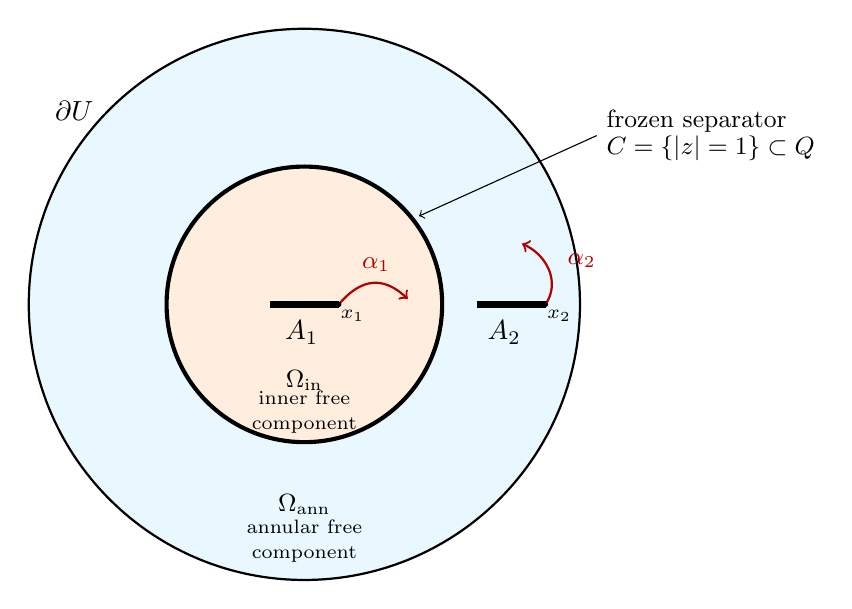
\begin{tikzpicture}[scale=1.75]
% free components, lightly shaded in different tints
\fill[cyan!9,even odd rule] (0,0) circle (2) (0,0) circle (1);
\fill[orange!13] (0,0) circle (1);
% localization boundary
\draw[thick] (0,0) circle (2);
\node at (140:2.18) {$\partial U$};
% the frozen separator, drawn bold
\draw[line width=1.5pt] (0,0) circle (1);
\draw[<-,shorten <=1.5pt] (38:1.02) -- (30:2.45)
  node[right,align=left] {\small frozen separator\\[-2pt]\small $C=\{|z|=1\}\subset Q$};
% atoms
\draw[line width=2.6pt] (-0.25,0) -- (0.25,0);
\node[below] at (-0.02,-0.05) {$A_1$};
\draw[line width=2.6pt] (1.25,0) -- (1.75,0);
\node[below] at (1.45,-0.05) {$A_2$};
% port arcs, one inside each free component
\draw[->,thick,red!70!black] (0.25,0) .. controls (0.42,0.20) and (0.58,0.20) .. (0.75,0.04);
\node[above,red!70!black] at (0.52,0.17) {\small $\alpha_1$};
\fill (0.25,0) circle (0.55pt);
\node[below right,inner sep=1pt] at (0.24,-0.02) {\scriptsize $x_1$};
\draw[->,thick,red!70!black] (1.75,0) .. controls (1.86,0.16) and (1.76,0.36) .. (1.58,0.44);
\node[right,red!70!black] at (1.84,0.32) {\small $\alpha_2$};
\fill (1.75,0) circle (0.55pt);
\node[below right,inner sep=1pt] at (1.74,-0.02) {\scriptsize $x_2$};
% component labels
\node at (0,-0.55) {\small $\Omega_{\mathrm{in}}$};
\node[align=center] at (0,-0.78) {\scriptsize inner free\\[-3pt]\scriptsize component};
\node at (0,-1.45) {\small $\Omega_{\mathrm{ann}}$};
\node[align=center] at (0,-1.72) {\scriptsize annular free\\[-3pt]\scriptsize component};
\end{tikzpicture}
\caption{The separation example of Example~\ref{ex:no-common-component}. The Jordan
localization is the disk $U=\{|z|<2\}$; the frozen inventory consists of the two atoms
$A_1=[-\frac14,\frac14]$ and $A_2=[\frac54,\frac74]$ and the bold circle $C$, a
frozen separator belonging to $Q$. The free domain $\Omfree=U\setminus Q$ has
exactly two components, shaded in different tints: the inner component
$\Omega_{\mathrm{in}}$ and the annular component $\Omega_{\mathrm{ann}}$. Each atom has
a singleton port arc ($\alpha_1$, $\alpha_2$) into its own component, so every
individual-access audit passes; but no single component ports to both atoms, so by
Theorem~\ref{thm:free-component} no protected ribbon-routing certificate exists, and by
the persistence clause no monotone connector enlargement inside $U$ can repair the
failure while $C$ stays in the frozen inventory.}
\label{fig:separation}
\end{figure}
